
\documentclass[10pt]{beamer}
\usepackage{amsmath}
\usepackage{mathtools}
\usepackage{multimedia}
\usepackage{hyperref}


\usefonttheme{professionalfonts} % using non standard fonts for beamer
\usefonttheme{serif} % default family is serif
%\documentclass[12pt]{beamerthemeSam.sty}
\usepackage{epsf}
%\usepackage{pstricks}
%\usepackage[orientation=portrait,size=A4]{beamerposter}
\geometry{paperwidth=160mm,paperheight=120mm}
%DT favorite definitions
\def\LL{\left\langle}	% left angle bracket
\def\RR{\right\rangle}	% right angle bracket
\def\LP{\left(}		% left parenthesis
\def\RP{\right)}	% right parenthesis
\def\LB{\left\{}	% left curly bracket
\def\RB{\right\}}	% right curly bracket
\def\PAR#1#2{ {{\partial #1}\over{\partial #2}} }
\def\PARTWO#1#2{ {{\partial^2 #1}\over{\partial #2}^2} }
\def\PARTWOMIX#1#2#3{ {{\partial^2 #1}\over{\partial #2 \partial #3}} }

\def\rightpartial{{\overrightarrow\partial}}
\def\leftpartial{{\overleftarrow\partial}}
\def\diffpartial{\buildrel\leftrightarrow\over\partial}

\def\BC{\begin{center}}
\def\EC{\end{center}}
\def\BN{\begin{enumerate}}
\def\EN{\end{enumerate}}
\def\BI{\begin{itemize}}
\def\EI{\end{itemize}}
\def\BE{\begin{displaymath}}
\def\EE{\end{displaymath}}
\def\BEA{\begin{eqnarray*}}
\def\EEA{\end{eqnarray*}}
\def\BNEA{\begin{eqnarray}}
\def\ENEA{\end{eqnarray}}
\def\EL{\nonumber\\}

\newcommand{\etal}{{\it et al.}}
\newcommand{\gbeta}{6/g^2}
\newcommand{\la}[1]{\label{#1}}
\newcommand{\ie}{{\em i.e.\ }}
\newcommand{\eg}{{\em e.\,g.\ }}
\newcommand{\cf}{cf.\ }
\newcommand{\etc}{etc.\ }
\newcommand{\atantwo}{{\rm atan2}}
\newcommand{\Tr}{{\rm Tr}}
\newcommand{\dt}{\Delta t}
\newcommand{\op}{{\cal O}}
\newcommand{\msbar}{{\overline{\rm MS}}}
\def\chpt{\raise0.4ex\hbox{$\chi$}PT}
\def\schpt{S\raise0.4ex\hbox{$\chi$}PT}
\def\MeV{{\rm Me\!V}}
\def\GeV{{\rm Ge\!V}}

%AB: my color definitions
%\definecolor{mygarnet}{rgb}{0.445,0.184,0.215}
%\definecolor{mygold}{rgb}{0.848,0.848,0.098}
%\definecolor{myg2g}{rgb}{0.647,0.316,0.157}
\definecolor{A}{rgb}{1.0,0.3,0.3}
\definecolor{B}{rgb}{0.0,1.0,0.0}
\definecolor{C}{rgb}{1.0,1.0,0.0}
\definecolor{D}{rgb}{0.5,0.5,1.0}
\definecolor{E}{rgb}{0.7,0.7,0.7}
\definecolor{abtitlecolor}{rgb}{1.0,1.0,1.0}
\definecolor{absecondarycolor}{rgb}{0.0,0.416,0.804}
\definecolor{abprimarycolor}{rgb}{1.0,0.686,0.0}
\definecolor{Red}           {rgb}{1,0.4,0.4}
\definecolor{Yellow}           {rgb}{1,1,0.0}
\definecolor{Grey}          {cmyk}{.7,.7,.7,0}
\definecolor{Blue}          {cmyk}{1,1,0,0}
\definecolor{Green}         {cmyk}{1,0,1,0}
\definecolor{Brown}         {cmyk}{0,0.81,1,0.60}
\definecolor{Silver}        {rgb}{0.95,0.9,1.0}
\definecolor{Sky}           {rgb}{0.07,0.0,0.2}
\definecolor{Darkbrown}     {rgb}{0.4,0.3,0.2}
\definecolor{40Gray}        {rgb}{0.4,0.4,0.5}
\usetheme{Madrid}


\setbeamercolor{normal text}{fg=Silver,bg=Sky}

%AB: redefinition of beamer colors
%\setbeamercolor{palette tertiary}{fg=white,bg=mygarnet}
%\setbeamercolor{palette secondary}{fg=white,bg=myg2g}
%\setbeamercolor{palette primary}{fg=black,bg=mygold}
\setbeamercolor{title}{fg=abtitlecolor}
\setbeamercolor{frametitle}{fg=abtitlecolor}
\setbeamercolor{palette tertiary}{fg=white,bg=Darkbrown}
\setbeamercolor{palette secondary}{fg=white,bg=absecondarycolor}
\setbeamercolor{palette primary}{fg=white,bg=40Gray}
\setbeamercolor{structure}{fg=abtitlecolor}

\setbeamerfont{section in toc}{series=\bfseries}

%AB: remove navigation icons
\beamertemplatenavigationsymbolsempty
\title[The seasons]{
  \textbf {The seasons}
}

\author [Astronomy 101]{Astronomy 101\\Syracuse University, Fall 2021\\Walter Freeman}

\date{\today}

\begin{document}



\frame{\titlepage}

\frame{\frametitle{\textbf{Announcements}}
\Large
\BI
%\item Paper 1 has been assigned (and we'll talk about it)
%\item If you want to get a head start on studying for Exam 1, the study guide is up
\item The prelab is posted online, but we haven't printed it because our printers have all failed.
\item We'll have copies for you ASAP, but in the meantime you can print it.
\item Please be careful when we are passing out today's exercise; I had to staple them by hand
\EI
}


\frame{\frametitle{\textbf{The tilt of the Earth's axis}}
\BC\Large
The Earth's axis of rotation is not lined up with its orbital axis. \\

\bigskip

It's tilted by 23.4 degrees.

\bigskip

The axis of rotation changes {\color{Red}only very slowly} (over millennia).

\EC

\bigskip
\bigskip

\BC
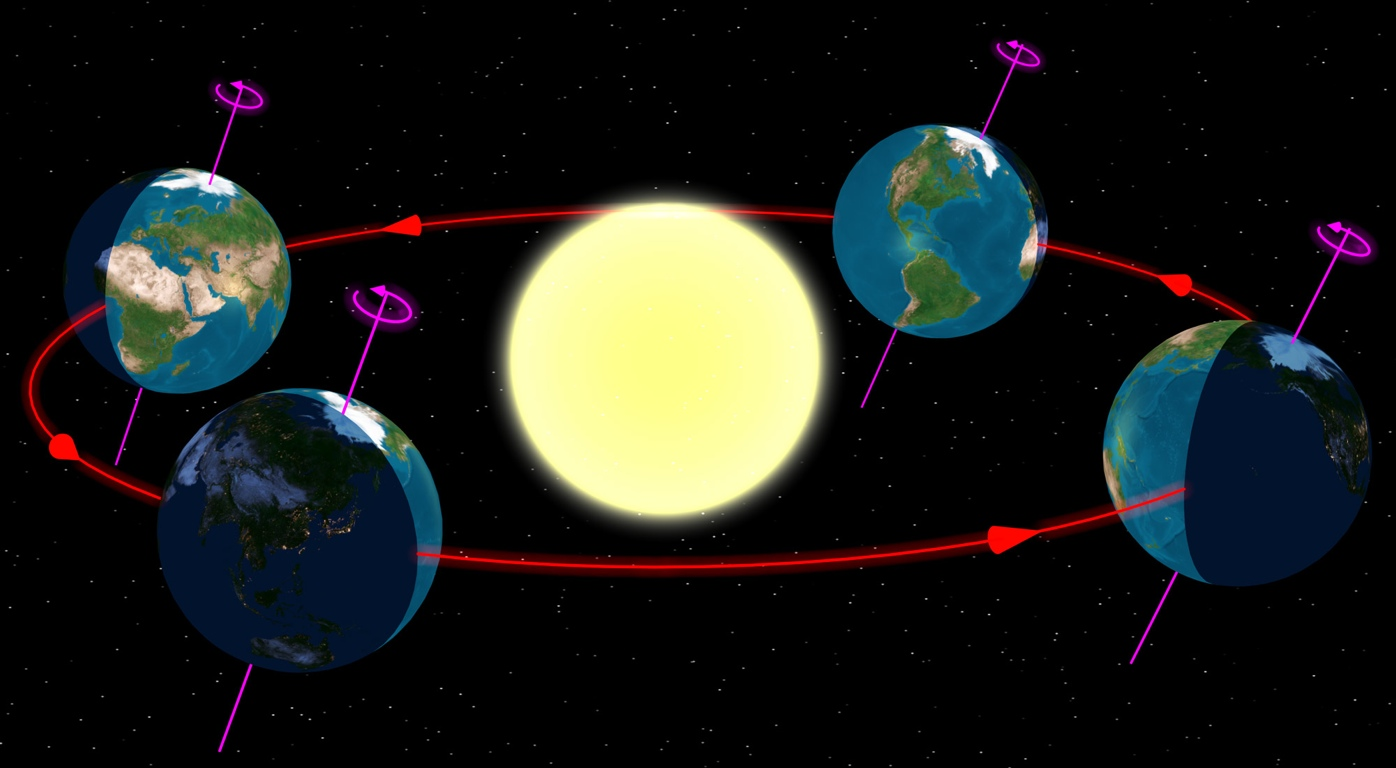
\includegraphics[width=0.8\textwidth]{axial-tilt.jpg}
\EC
}

\frame{\frametitle{\textbf{Let's look at the consequences of this}}

}


\frame{\frametitle{\textbf{What consequences does this have for the sky?}}

\Large

As the year progresses, thinking only about noon, will the Sun:

\Large

\bigskip
\bigskip
\bigskip

I. Move higher and lower in the sky \\
II. Move east/west relative to the stars

\bigskip
\bigskip
\bigskip

\Huge

\color{A}A: I only \\
\color{B}B: II only \\
\color{C}C: I and II \\
\color{D}D: None of the above 

}


\frame{\frametitle{\textbf{A demonstration in Stellarium}}
\Large
Let's use {\it Stellarium} to examine the Sun at different times of year.

\bigskip
\bigskip
\bigskip


Notice:
\BI
\item{The Sun is higher or lower in the sky depending on the time of year}
\item{The Sun moves westward with respect to the stars:} 
\BI
\item{Every {\it solar day}, the Sun's east/west position (azimuth) stays fixed, but the stars move {\color{Red}East}}
\item{Every {\it sidereal day}, the stars' position stays fixed, but the Sun moves {\color{Red}West}}
\pause
\item{``One solar day is a bit more than one sidereal day''}
\item{``One sidereal day is a bit less than one solar day''}
\EI
\EI
}

\frame{\frametitle{\textbf{The solstices and equinoxes}}
\Large
We give special names to the points in Earth's orbit where the Earth's axis is tilted directly toward/away from the Sun:

\bigskip
\bigskip

\BC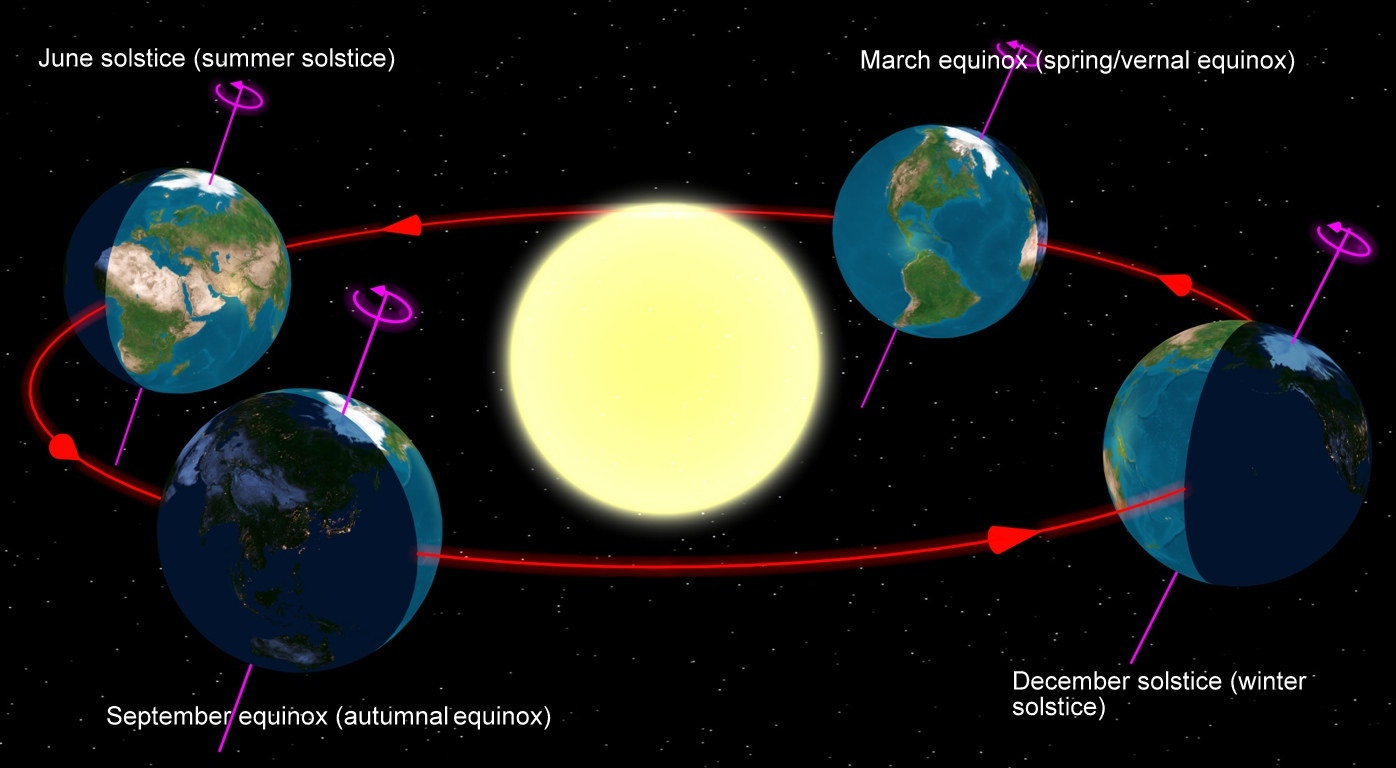
\includegraphics[width=0.8\textwidth]{solstices.jpg}\EC
}

\frame{\frametitle{\textbf{The solstices and equinoxes}}
\Large
\BC
Many cultures have ascribed significance to the annual movement of the Sun. \\

\bigskip
\bigskip

Perhaps the most famous artifact of this is Stonehenge:

\bigskip
\bigskip

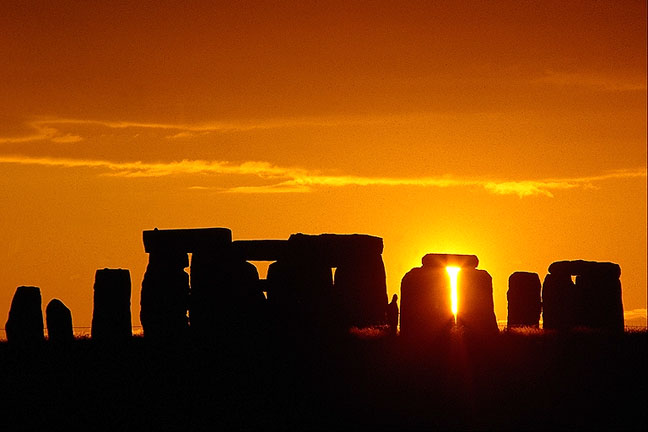
\includegraphics[width=0.6\textwidth]{stonehenge.jpg}

\EC

}



\frame{\frametitle{\textbf{The tropics}}

\BC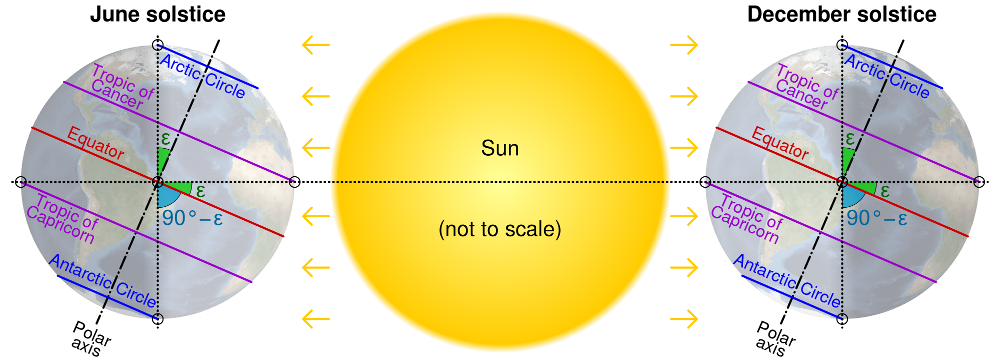
\includegraphics[width=0.6\textwidth]{circle.png}\EC

\bigskip
\bigskip
\bigskip

\Large

The region on Earth where the Sun alternates between the northern sky and the southern sky is called the 
{\color{Red} tropics}.

\bigskip
\bigskip
\large
\BI
\item{The northern boundary is called the {\color{Red}Tropic of Cancer}}
\item{The southern boundary is called the {\color{Red}Tropic of Capricorn}}
\item{These occur at $23.4^\circ$ N/S latitude}
\EI

On the June solstice, the sun reaches the zenith along the Tropic of Cancer.

On the December solstice, the sun reaches the zenith along the Tropic of Capricorn.
}



\frame{\frametitle{\textbf{The Arctic and Antarctic}}

\BC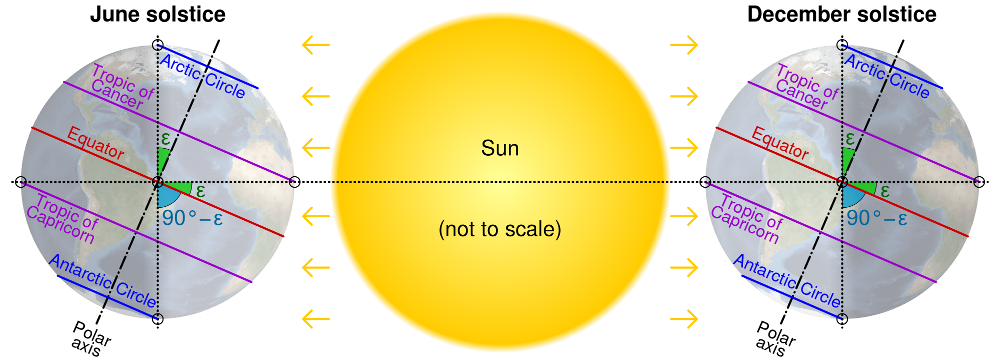
\includegraphics[width=0.6\textwidth]{circle.png}\EC

\bigskip
\bigskip

\Large
The region where the sun either never rises or never sets during part of the year 
is called the Arctic (north) or Antarctic (south).



\bigskip

\BI
\item{North of the Arctic Circle, the sun never rises on the December solstice, and never sets on the June solstice.}
\item{South of the Antarctic Circle, the sun never sets on the December solstice, and never rises on the June solstice.}
\item{These occur at $90-23.4^\circ = 66.6$ N/S latitude}
\EI
}




\frame{\frametitle{\textbf{What consequences does this have on Earth?}}
\Large
Thinking only about noontime (when the sun is highest in the sky), will the sun ever reach the zenith in Syracuse (latitude $43^\circ$ N)?

\bigskip
\bigskip
\bigskip
\bigskip

\color{A}A: Yes \\
\color{B}B: No \\
}

\frame{\frametitle{\textbf{What consequences does this have on Earth?}}
\Large
Thinking only about noontime (when the sun is highest in the sky), will the sun ever reach the zenith in Lima, Peru (latitude $12^\circ$ S)?

\bigskip
\bigskip
\bigskip
\bigskip

\color{A}A: Yes \\
\color{B}B: No \\
}

\frame{\frametitle{\textbf{What consequences does this have on Earth?}}
\Large
Which is true about the Sun on June 21 in Svalbard  (latitude $78^\circ$ N)?

\bigskip
\bigskip
\bigskip
\bigskip

\color{A}A: It will never rise \\
\color{B}B: It will never set \\
\color{C}C: It will reach the zenith of the sky \\
\color{D}D: It will travel from east to west in the northern sky \\
\color{E}E: It will travel from east to west in the southern sky \\
}

\frame{\frametitle{\textbf{The seasons}}
\large
The tilt of the Earth toward/away from the Sun controls the amount of sunlight we get at different times of year!

\bigskip
\bigskip

This happens for two important reasons. Thinking about the Northern hemisphere...

\bigskip
\bigskip

\BI
\item{The Sun is visible in the sky for longer in June than in December}
\item{Sunlight strikes the Earth more directly in June than in December}
\EI

\BC
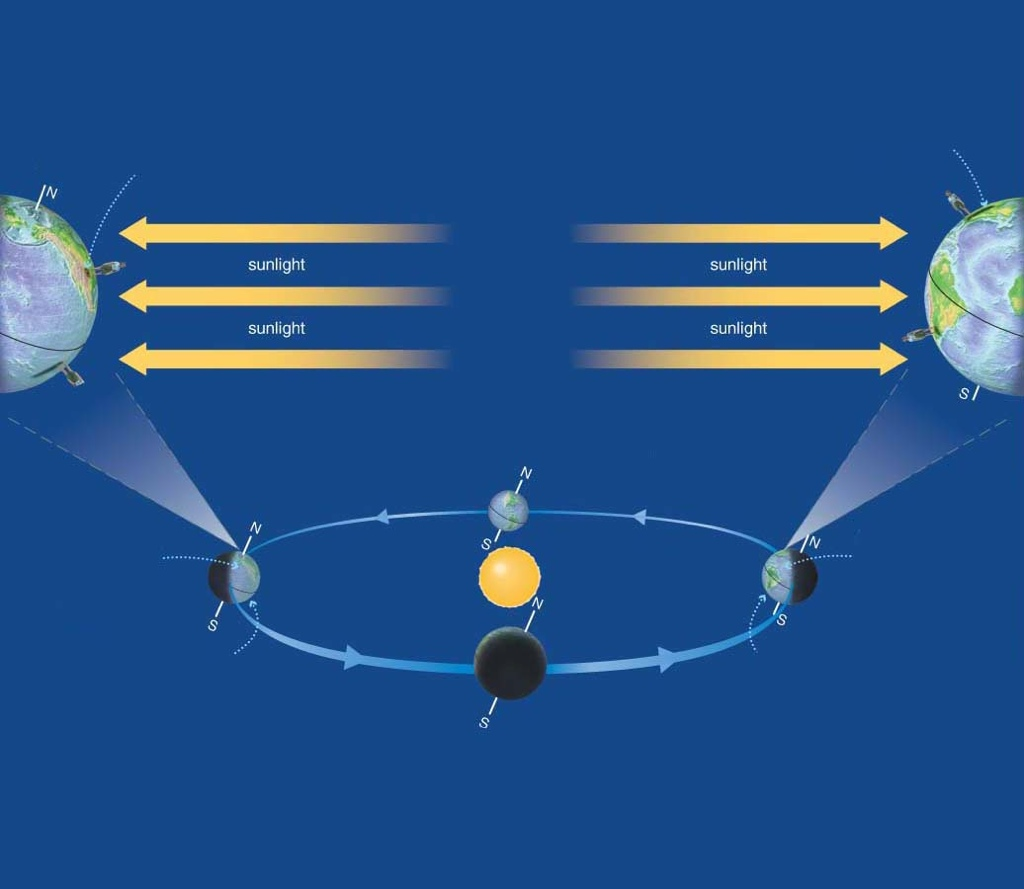
\includegraphics[width=0.5\textwidth]{sun-incidence.jpg}
\EC
}


\frame{\frametitle{\textbf{The seasons}}
\BC
\Huge
Complete the handout, and start on your homework if you want.


\vspace{1in}
\Large

After this, we will review the quiz.
\EC

}


\frame{\frametitle{\textbf{The seasons}}
\Large
\BC
This is why the Earth is hotter in summer. \\
It has {\color{Red}nothing} to do with the distance from the Sun!
\EC
}

\frame{

\Large
\begin{center}
Let's look at some questions from the quiz...
\end{center}
}

\end{document}
